\lez{20}{03-04-2020}{}
\subsection{Hole function o funzione di correlazione totale.}
\label{subsec:Hole function}
Abbiamo visto come la $g(r)$ esprima la probabilità di trovare una particella a distanza $r$ da un'altra, possiamo definire allo stesso modo un'altra quantità utile:
\begin{defn}[Hole function]{def:Hole function}
	\[\begin{aligned}
		h(r) 
		=&
		g(r)-1=\\
		=&
		\frac{1}{8\pi^3\rho }\int\left[ S(k)-1 \right]
		e^{-i \v{k}\v{r}}d \v{k} =\\
		=&
		\frac{1}{2\pi^2\rho r}
		\int_{0}^{\infty} \left[ S(k)-1 \right] 
		k\sin(kr)dk
	.\end{aligned}\]
\end{defn}
Mettiamo a confronto le funzioni $S(q)$ e $g(r)$ per un fluido alla "Lennard Jones"\footnote{Ovvero formato da particelle che interagiscono soltanto con forze di Van der Wals.}: l'Argon \footnote{La scelta dell'Argon al posto dell'elio è dettata dal fatto che l'elio condensa a basse temperature.}.
\begin{figure}[H]
	\centering
	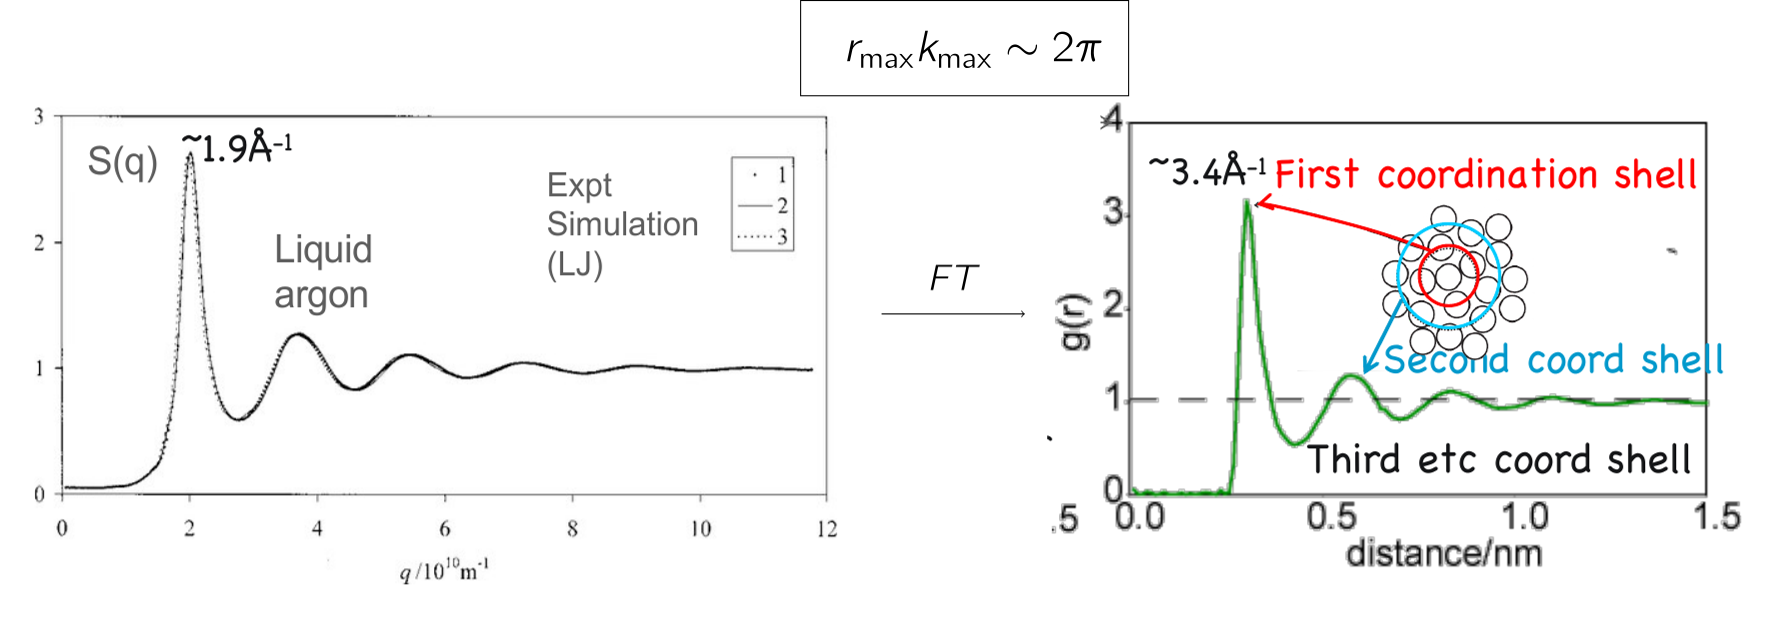
\includegraphics[width=0.8\textwidth]{figures/lennard-S.png}
	\caption{$S(q)$ e $g(r)$ per l'Argon.}
	\label{fig:-figures-lennard-S-png}
\end{figure}
Notiamo che nel limite di $q$ grande la funzione $S(q)$ tende ad 1, quindi facendo $S(q)-1$ ottengo una funzione che asintoticamente va a zero (uno dei requisiti per la $FT$).\\
Notiamo la somiglianza tra le due funzioni in spazio diretto e spazio reciproco, tuttavia dalle oscillazioni in $g(r)$ si riesce ad estrarre informazioni fisiche più intuitive:
\begin{description}
	\item[Diametro delle particelle del fluido] 
		In un fluido reale (non puntiforme) nelle strette vicinanze di una 
		particella avremo probabilità zero (quasi esatto) di trovare un'altra
		particella. Questo ci da una informazione del diametro della particella
		che compone il fluido.
	\item[Durezza delle particelle]
		La salita della $g(r)$ dopo la parte quasi nulla è proporzionale alla
		durezza delle particelle: particelle più dure avranno salita più ripida
		di particelle morbide.
	\item[Primo picco: shell di primi vicini]
		In un liquido non ci sono posizioni definite delle particelle, tuttavia 
		si preserva ancora un certo ordine locale: la shell di primi vicini è
		ancora ben definita (come testimonia l'altezza del primo picco).
	\item[Allontanandosi dalla prima shell svanisce l'ordine locale nel fluido]
		Questo lo si vede dal fatto che i picchi sono sempre meno marcati 
		all'aumentare di $r$. Nel limite di $r$ grande la $S(q)$ tende
		ad 1 come nel caso dei gas perfetti.
\end{description}
\subsection{Fattore di struttura statistica per un fluido poliatomico.}
\label{subsec:Fattore di struttura statistica per un cristallo poliatomica}
Nel caso di cristallo poliatomico (composto da specie $\alpha,\beta$) possiamo definire il fattore di struttura e la funzione di correlazione di coppia per ciascuna delle coppie $\alpha\beta$ all'interno della struttura:
\[
	S_{\alpha\beta}(k) - 1 =
	\rho \int\left[ g_{\alpha\beta}(r)-1 \right]e^{i \v{r}\v{k}}d \v{r}
.\] 
Ognuno di questi fattori può essere misurato separatamente sfruttando i diversi fattori di forma degli atomi differenti.
\subsection{Caso speciale: l'acqua.}
\label{subsec:Caso speciale: l'acqua.}
L'acqua è un caso speciale di fluido poliatomico poiché è uno dei sistemi più incasinati che ci siano, il suo diagramma di fase è il seguente:
\begin{figure}[H]
	\centering
	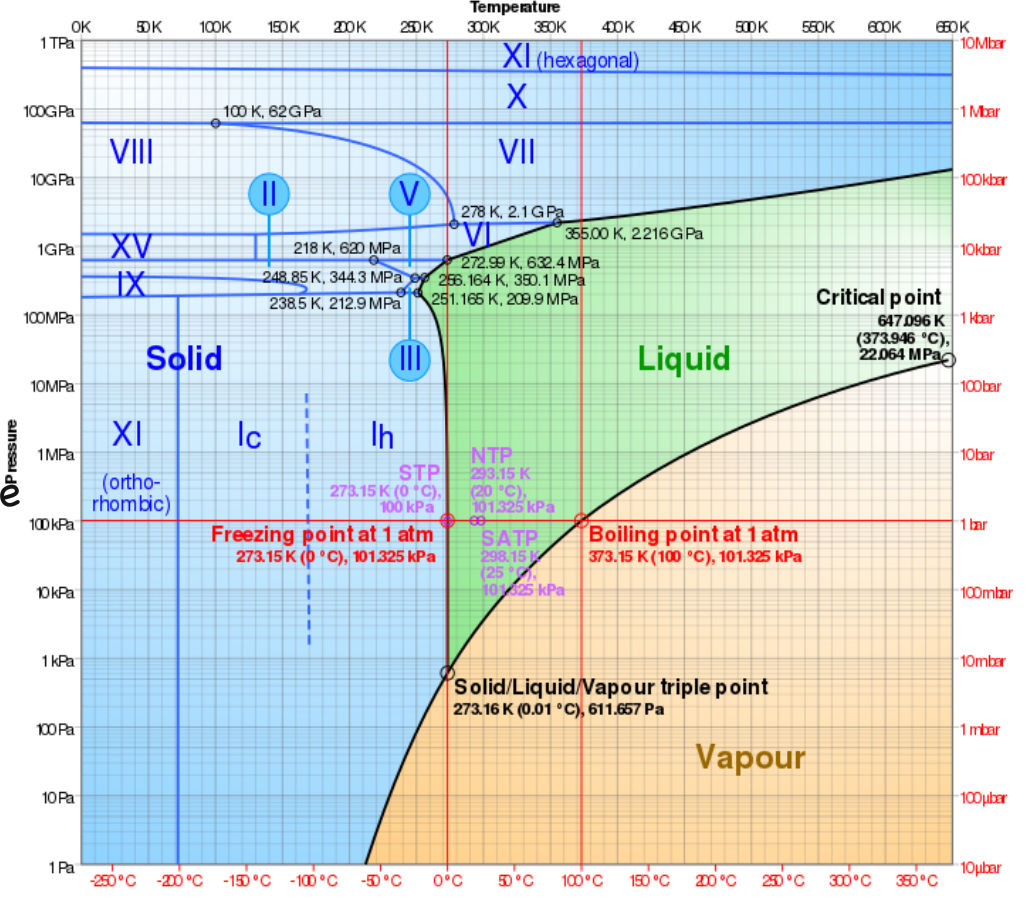
\includegraphics[width=0.6\textwidth]{figures/acqua-fase.png}
	\caption{Diagramma di fase dell'acqua.}
	\label{fig:figures-acqua-fase-png}
\end{figure}
Per trovare il fattore di struttura "relativo" per gli atomi che compongono l'acqua si può procedere nel seguente modo:
\begin{itemize}
	\item 
		Facendo uno scattering con i raggi X non vediamo l'idrogeno: 
		vediamo solo l'ossigeno \footnote{In questo modo si riesce a vedere
		la nube elettronica e dedurre la posizione degli atomi.}.
	\item 
		Facendo uno scattering con i neutroni, sensibili ai diversi atomi e
		isotopi: si fanno sostituzioni isotopiche (acqua pesante) e si guardano 
		le differenze deducendo la struttura.
\end{itemize}
Il risultato di queste tecniche è riportato in figura \ref{fig:S-acqua}.
\begin{figure}[ht]
	\centering
	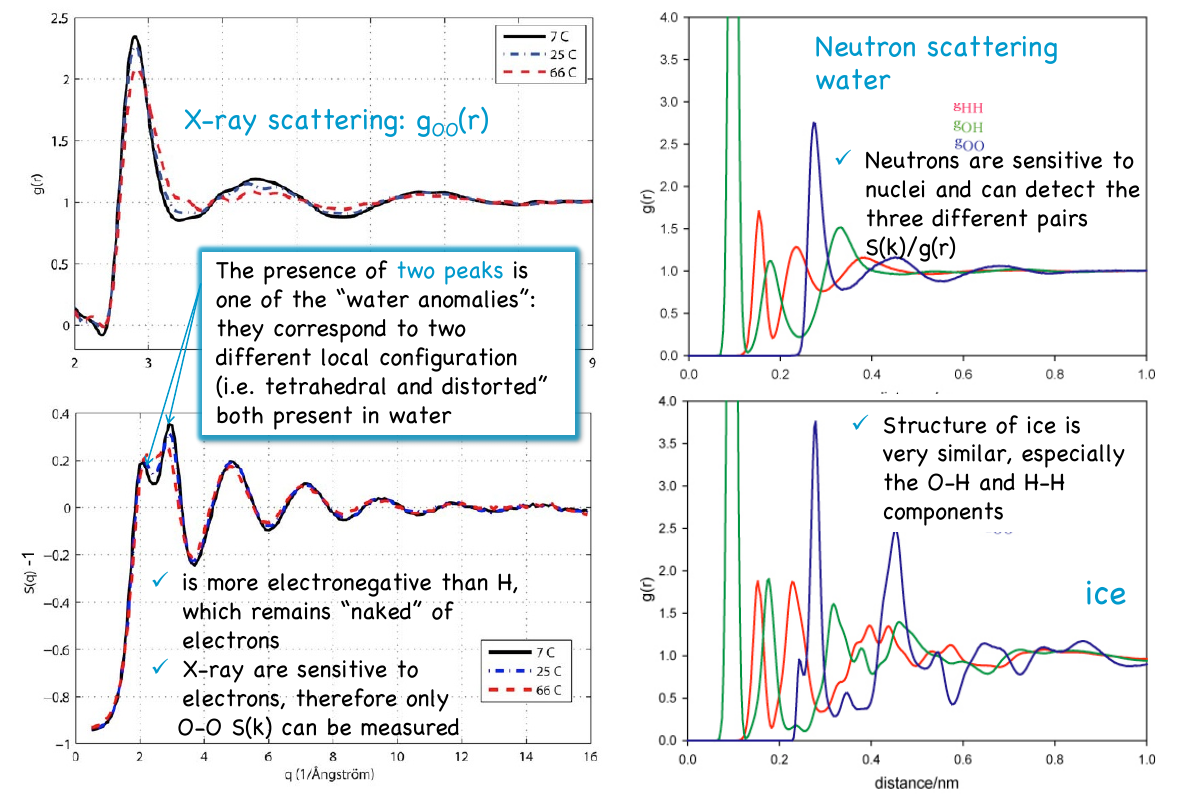
\includegraphics[width=0.7\textwidth]{figures/S-acqua.png}
	\caption{Fattori di struttura statica per l'acqua.}
	\label{fig:S-acqua}
\end{figure}
Da tale figura possiamo capire la complessità della molecola. Nel plot in basso a destra è evidente una anomalia nella $S_{O-O}(q)$: un doppio picco. Questa è legata al fatto che l'acqua ha una doppia configurazione locale: tetraedrica e caotica.\\
Lo scattering di elettroni riportato invece a destra (per acqua sopra e per ghiaccio sotto). Tale scattering ci mostra come le forti correlazioni presenti all'interno dell'acqua liquida si conservino parzialmente anche all'interno del ghiaccio.\\
La cosa importante è che anche all'interno dell'acqua liquida abbiamo una forte correlazione tra gli atomi, molto simile a quella che si ha nel ghiaccio (con la grande differenza che sono in due stati fisici diversi!).\\
Possiamo dare una spiegazione a questo fatto grazie ai ponti ad idrogeno, tali ponti stabilizzano sia l'acqua che il ghiaccio usando gli H come ponte tra i vari ossigeni.\\
L'ossigeno ha infatti in totale 6 elettroni di valenza, ne condivide 2 con l'idrogeno. È quindi circondato da 4 doppietti elettronici che si dispongono in sp3: ai vertici di un tetraedro. \\
Essendo l'ossigeno "nudo" di carica negativa (quindi parzialmente carico +) potrà formare un legame direzionale con i doppietti elettronici ai vertici del tetraedro. Questa interazione forma il legame ad idrogeno che è poco più debole di un legame covalente ma comunque direzionale. \\
Questo conferisce all'acqua tutte le proprietà macroscopiche anomale (come le densità massima nell'acqua).\\
Tutte queste considerazioni si possono fare analizzando il grafico delle $g(r)$, quindi possiamo capire l'importanza di questo tipo di analisi.
\subsection{Analisi della $g(r)$ dell'Argon}
\label{subsec:Analisi della $g(r)$ dell'argon liquido}
\subsubsection{Argon liquido}
\label{subsubsec:Argon liquido}
Nella Figura \ref{fig:figures-argon-g-png} possiamo vedere la $g(r)$ dell'Argon liquido a diverse temperature.
\begin{figure}[ht]
	\centering
	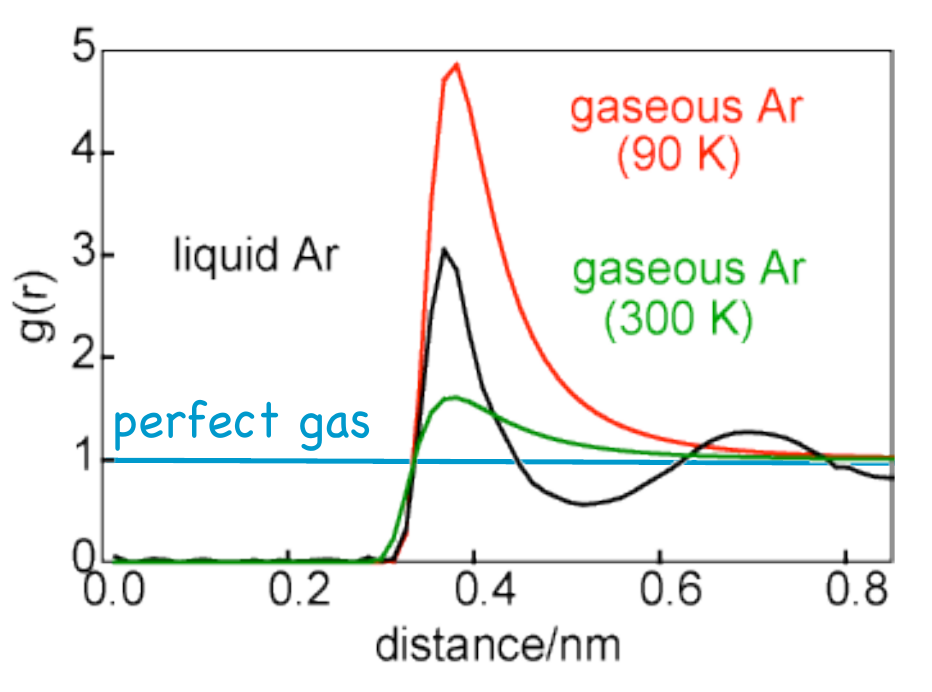
\includegraphics[width=0.4\textwidth]{figures/argon-g.png}
	\caption{Grafico della $g(r)$ per l'Argon gassoso e liquido.}
	\label{fig:figures-argon-g-png}
\end{figure}
In questo grafico è evidente tutto quello affermato nella lezione: il gas perfetto ha un andamento costante e unitario, man a mano che la temperatura diminuisce viene fuori la struttura periodica dell'Argon.
\subsubsection{Argon solido}
\label{subsubsec:Argon solido}
Nell'argon solido abbiamo dei picchi dalla forma gaussiana come possiamo vedere in Figura \ref{fig:-solid-Argon}. 
\begin{figure}[ht]
	\centering
	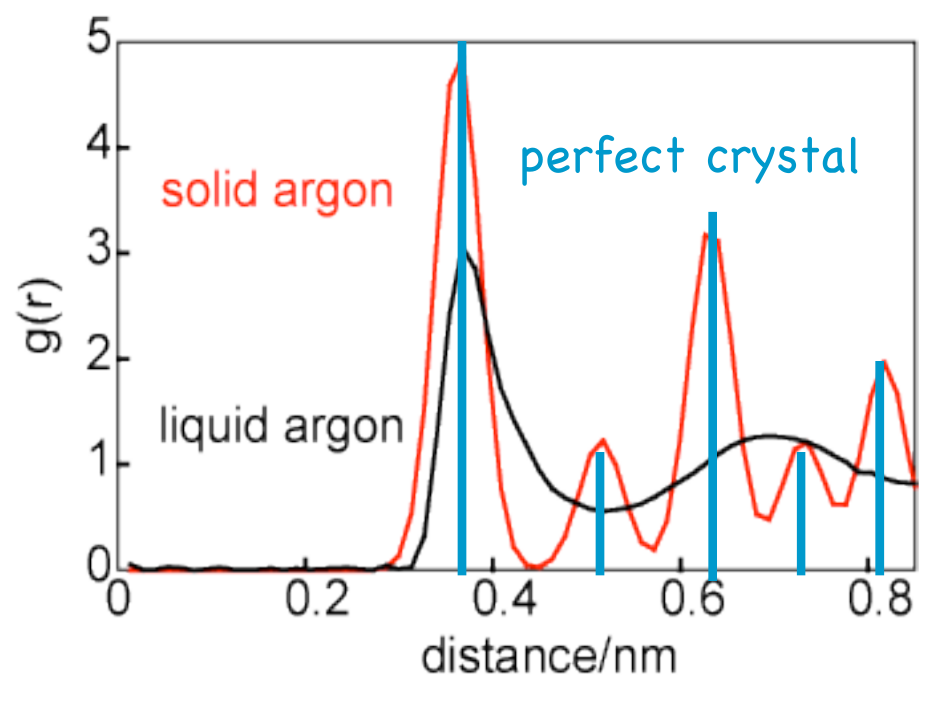
\includegraphics[width=0.45\textwidth]{figures/argon-g-solido.png}
	\caption{Grafico della $g(r)$ per l'Argon solido e liquido.}
	\label{fig:-solid-Argon}
\end{figure}
In questo caso infatti abbiamo che 
\[
	g(\v{r}_1,\v{r}_2) \propto \rho (\v{r}_1)\rho (\v{r}_2)
.\] 
Il primo picco inoltre è collocato approssimativamente nella stessa posizione del picco presente nello stato liquido e corrisponde alla shell di primi vicini. 
Notiamo anche che se il cristallo fosse perfetto (atomi perfettamente localizzati) allora il plot della $g(r)$ sarebbe formato da delle $\delta$ corrispondenti ai picchi gaussiani come quelli nella figura.\\
Questi picchi non possono essere raggiunti come $\delta$ nemmeno a temperatura nulla poiché, come sappiamo, anche in questo caso vi sarebbero delle fluttuazioni.
\subsection{Struttura dell'argon e funzione $g(r)$.}
\label{subsec:Struttura dell'argon e funzione $g(r)$.}
Solitamente di fluidi di Lennard Jones solidificano in un cristallo avente celle FCC (cubico facce centrate), tali celle sono quelle più compatte possibile e hanno una forma del tipo:
\begin{figure}[H]
	\centering
	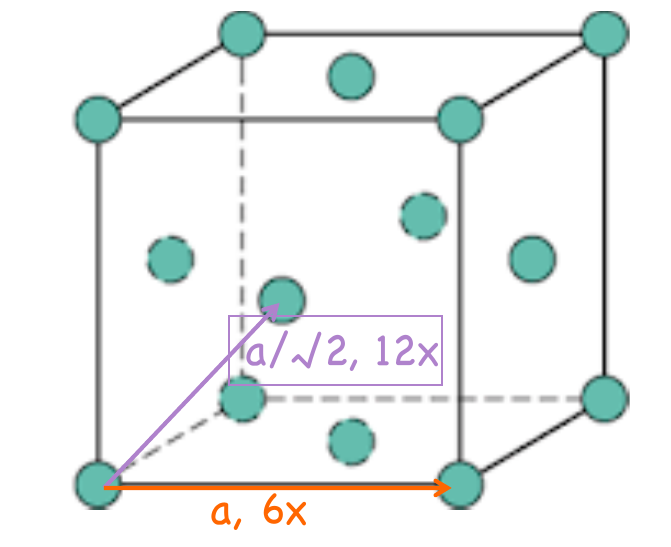
\includegraphics[width=0.3\textwidth]{figures/FCC.png}
	\caption{Struttura FCC.}
	\label{fig:figures-FCC-png}
\end{figure}
\noindent
Mettendoci a cavallo di uno di questi atomi possiamo vedere a che distanza e quante volte incontriamo un atomo vicino. Il conteggio è riportato in Figura \ref{fig:figures-FCC-png}, sovrapposta alla forma della cella.\\
Vediamo allora che nella $g(r)$ si ha un primo picco proprio in corrispondenza dell'atomo vicino "più conteggiato". \\
In particolare si ha che l'altezza di un picco è proporzionale a $n/r^2$ in cui $n$ è il numero di atomi vicini a distanza $r$. \\
Un esercizio interessante potrebbe essere quello di prendere una cella cubica di forma a piacimento (FCC, BCC, ecc..) e provare a calcolare l'altezza dei picchi e la loro distanza.
Una volta fatto questo prendere una funzione formata da tante $\delta$ della stessa altezza dei picchi e distanti l'una dall'altra come questi ultimi. 
Successivamente si può fare un prodotto di convoluzione di queste $\delta$ con delle gaussiane anche esse localizzate ed ottenere una buona stima di $g(r)$ per la nostra struttura (come si nota dalla Figura \ref{fig:FCC-argon-plot}).\\
\begin{figure}[ht]
	\centering
	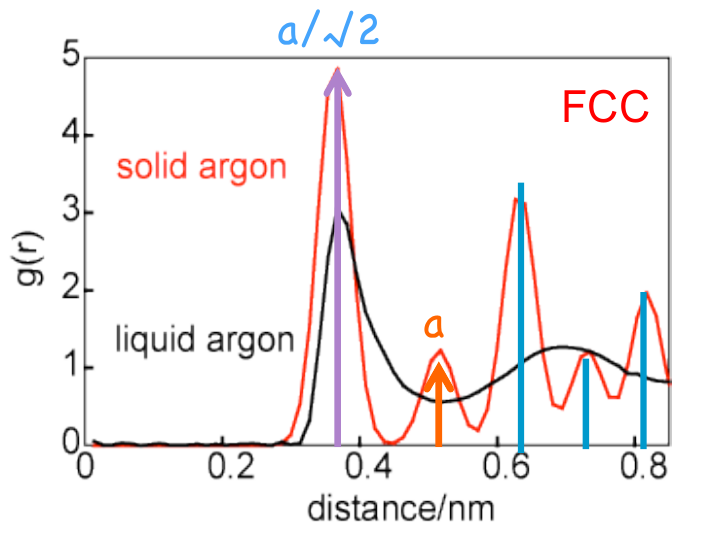
\includegraphics[width=0.4\textwidth]{figures/FCC-plot.png}
	\caption{$g(r)$ per un cristallo di Argon FCC.}
	\label{fig:FCC-argon-plot}
\end{figure}
Notiamo anche che più ci si allontana dalla shell dei primi vicini e più i picchi si avvicinano tra loro, vediamo che asintoticamente la $g(r)$ tende ad uno, poiché i picchi si infittiscono e scalano come $\left( 4\pi r^2 \right)^{-1}$.\\
Inoltre abbiamo che più il cristallo di forma e più tra un picco e l'altro di formeranno degli zeri, l'andamento al calare della temperatura tende ad avvicinarsi a quello delle $\delta.$ \\
Per l'Argon abbiamo parlato fin'ora della $g(r)$, vediamo adesso come va la $S(q)$ al variare dello stato del sistema di Lennard Jones.
\subsection{Diagrammi di stato e $S(q)$}
\label{subsec:Diagrammi di stato e $S(q)$}
Un tipico diagramma di fase per un sistema di Lennard Jones è il seguente:
\begin{figure}[H]
	\centering
	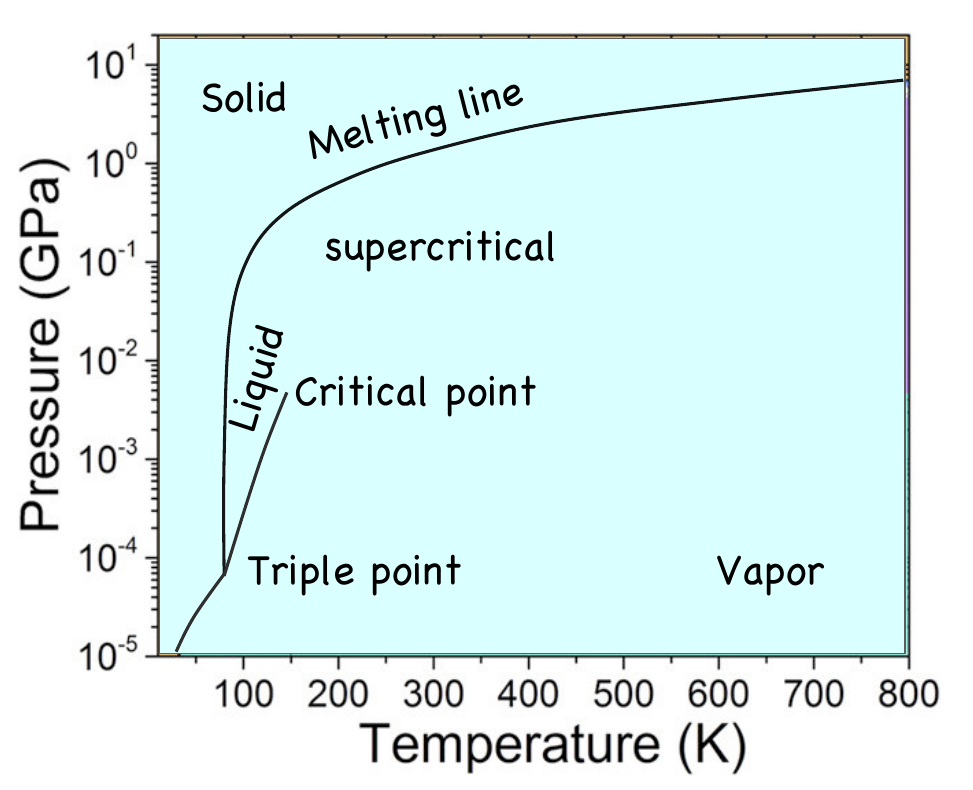
\includegraphics[width=0.5\textwidth]{figures/fase-lennard-jones.png}
	\caption{Diagramma di fase per sistema di Lennard Jones.}
	\label{fig:figures-fase-lennard-jones-png}
\end{figure}
\noindent
In tali sistemi abbiamo generalmente un punto triplo ed un punto critico. Ricordiamo che il punto critico è il punto al di sopra del quale, diminuendo la temperatura, non si ottiene più una discontinuità in densità della materia, quindi non si può parlare di avvenuto passaggio di stato. \\
In realtà sono presenti cose più particolari a livello dinamico al di sopra del punto critico, esiste infatti una linea detta \textit{linea di Frenkel}. Questa linea delimita una transizione del secondo ordine: non vi è associato alcun calore latente.\\
Notiamo inoltre dalla Figura \ref{fig:figures-slide-tesi-png} che la $S(k=0)$ non è nulla ed il suo andamento dipende dalla posizione nel diagramma di stato che andiamo a modificare.
\begin{figure}[ht]
	\centering
	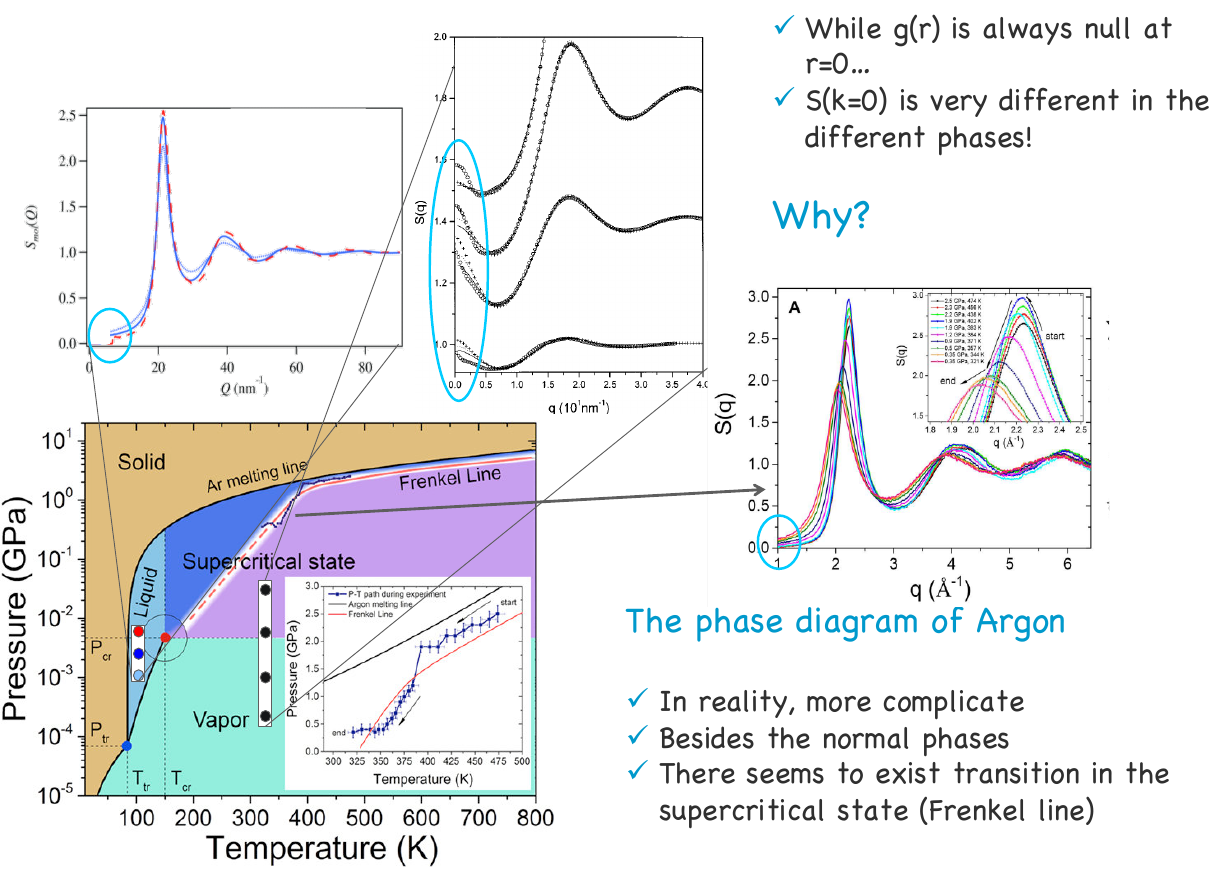
\includegraphics[width=0.9\textwidth]{figures/slide-tesi.png}
	\caption{Andamento della $S(q)$ per varie posizioni del diagramma di stato.}
	\label{fig:figures-slide-tesi-png}
\end{figure}
\subsection{Relazione di Ornstein-Zernike}
\label{subsec:Relazione di Ornstein-Zernike}
Vediamo qual'è il significato di $S(q)$ con $q\to 0$. Tale funzione calcolata in 0 è:
\[\begin{aligned}
	S(k=0)
	=&
	1+\rho \int\left[ g(r)-1 \right] =\\
	=&
	1 + \frac{1}{N} \int\int 
	\underbrace{
	\rho ^2g(r)d 
	}_{\overline{\rho }_2(\v{r}.\v{r}')}
	\v{r}d \v{r}'
	-
	\rho \int d \v{r}
.\end{aligned}\]
Ricordando che:
\[
	\int\int \overline{\rho }_2(\v{r},\v{r}')d \v{r} d \v{r}'
	=
	\left<N^2 \right>- \left<N \right>
.\] 
Possiamo risolvere in $N$:
\[\begin{aligned}
	S(k=0)
	=&
	1 + \frac{\left<N^2\right> - \left<N \right>}{\left<N \right>} - \left<N \right>=\\
	=&
	\frac{\left<N^2 \right>-\left<N \right>^2}{\left<N \right>} =\\
	=&
	\frac{\left<\Delta N^2 \right>}{\left<N \right>}
	\label{eq:Orne2}
.\end{aligned}\]
Quindi abbiamo che il valore del fattore di struttura statica in $\Delta\v{k}=0$ è collegato alle fluttuazioni del valore medio del numero di particelle relativo.\\
In particolare si ha in un cristallo, dove il numero di particelle non varia, che $S(k)$ si annulla per $k=0$. \\
Vediamo se questa caratteristica è collegata a qualche proprietà macroscopica della materia. Per far questo mettiamoci nel sistema del gran canonico:
\[\begin{aligned}
	&N = -\left.\frac{\partial \Omega }{\partial \mu} \right|_{T,V}\\
	& \left<\Delta N^2 \right> = kT\left.\frac{\partial N}{\partial \mu} \right|_{T,V}
		\label{eq:Nemu}
.\end{aligned}\]
Possiamo riscrivere la seconda collegandola al teorema di Fluttuazione-Dissipazione:
\[
	\left<\Delta M^2 \right>=kT\left.\frac{\partial M}{\partial H} \right|_{T,V}
.\] 
Dove $\Delta M$ sono le fluttuazioni di una determinata variabile (come la magnetizzazione) mentre $H$ è il campo esterno che genera tale variabile (nel caso del della magnetizzazione il campo magnetico) \footnote{Questa è la forma statica del teorema, scriveremo la generale più avanti.}. \\
Possiamo notare dalle equazioni in \ref{eq:Nemu} che $N $ e $\mu$ sono due variabili legate tra loro esattamente come $M$ e $H$ nella notazione del teorema. In un certo senso il potenziale chimico è il campo esterno che mi fa cambiare il numero di particelle.\\
Maneggiamo a questo punto la seconda equazione in \ref{eq:Nemu}:
\[\begin{aligned}
	\left<\Delta N^2 \right> 
	=&
	kT 
	\frac{\left.\frac{\partial N}{\partial P} \right|_{T,V}}
		{\left.\frac{\partial \mu}{\partial P} \right|_{T,V}}=\\
	=&
	kT \frac{\left.\frac{\partial N}{\partial P} \right|_{T,V}}{\frac{1}{\rho }}=\\
	=&
	V \rho kT \left.\frac{\partial \rho }{\partial P} \right|_{T,V}=\\
	=&
	V\rho ^2kT 
	\underbrace{
	\frac{1}{\rho }\left.\frac{\partial \rho }{\partial P} \right|_{T,V}
	}_{k_{_T}}
	\label{eq:Orne1}
.\end{aligned}\]
Il secondo passaggio è stato ottenuto grazie ad un differenziale (che probabilmente abbiamo già affrontato):
\begin{fact}[Relazione di Gibbs-Duheim]{fact:Relazione di Gibbs-Duheim}
	\[
		N  d \mu + S dT - V dP = 0
	.\]
	Dalla quale abbiamo preso:
	\[
		\left.\frac{\partial \mu}{\partial P} \right|_{T,V}
			=
			\frac{V}{N} 
			=
			\frac{1}{\rho}
	.\] 
	Il differenziale in questione può essere ottenuto differenziando una delle
	qualunque energie libere, ad esempio quella di Gibbs.
\end{fact}
Mettendo insieme la \ref{eq:Orne2} e la  \ref{eq:Orne1} otteniamo una importante relazione (molto molto importante all'esame):
\begin{fact}[Relazione di Ornstein-Zernike]{fact:Relazione di Ornstein-Zernike}
	\[
		\lim_{k \to 0} S(k) = \rho kT k_{_{T}}
	.\] 
\end{fact}
L'importanza di questa relazione è evidente: abbiamo legato il limite per $k\to 0$ di $S(k)$ alla comprimibilità isoterma. Se la comprimibilità di un materiale è nulla (come avviene (quasi) nei cristalli) allora si annulla asintoticamente anche la $S(k)$.
\subsection{Limite asintotico di $S(K)$ nel caso di Gas perfetti}
\label{subsec:Limite asintotico di $S(K)$ nel caso di Gas e liquidi}
Nel caso di un gas abbiamo una comprimibilità pari a :
\[\begin{aligned}
	k_{_T} =& \frac{1}{\rho }\frac{\partial \rho }{\partial P} =\\
	=&
	\frac{1}{\rho }\frac{\partial N/V}{\partial P}
	\xrightarrow[]{PV=NkT} \frac{1}{\rho } \frac{\partial P /kT}{\partial P} 
.\end{aligned}\]
Quindi utilizzando l'equazione del gas perfetto abbiamo che:
\[
	k_{_T} = \frac{1}{\rho kT}
.\] 
Per questo motivo per un gas perfetto utilizzando la Relazione \ref{fact:Relazione di Ornstein-Zernike} si ottiene che:
\[
	S(q=0)=1
.\] 
In linea con quanto detto fin'ora.
\subsection{Limite asintotico di $S(K)$ nel caso di plasmi}
\label{subsec:Limite asintotico di $S(K)$ nel caso di plasmi}
Consideriamo un fluido di particelle cariche non interagenti su un fondo di carica positivo neutralizzante inerte (Fluido di Wiegner):
\begin{figure}[H]
	\centering
	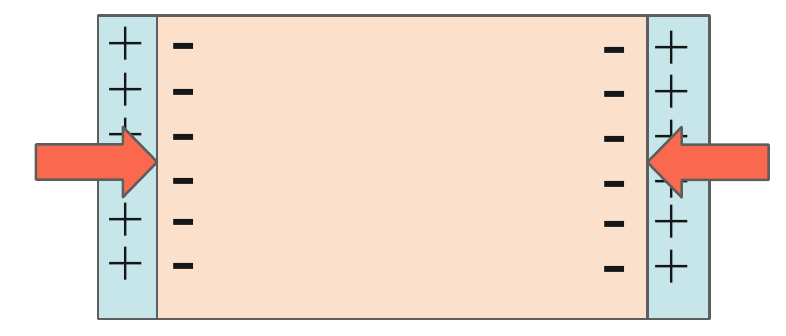
\includegraphics[width=0.4\textwidth]{figures/Plasma-schiacciato.png}
	\caption{Plasma compresso.}
	\label{fig:figures-Plasma-schiacciato-png}
\end{figure}
Quando comprimo il fondo di carica non altera le sue caratteristiche fisiche, la parte negativa (corrispondente ad esempio ad un gas di elettroni) invece permette la formazione di separazione di carica ai bordi. Questa separazione crea dei campi macroscopici, quindi abbiamo che
\[
	\lim_{k \to 0} S(k) = -\frac{kT}{\rho }\chi(k, \omega = 0)
.\] 
Dove abbiamo messo $\omega = 0$ supponendo di essere nel limite statico ed avendo generalizzato la compressibilità alla funzione di risposta lineare.\\
Nel caso del gas in questione tale funzione è la funzione di risposta dielettrica, questa può essere ottenuta risolvendo l'equazione di Poisson con le condizioni al contorno (in modo naif per un condensatore piano). Risolvendo si ha:
\[
	\lim_{k \to 0} S(k) = \frac{kT}{4\pi\rho e^2}k^2
.\] 
Quindi va a zero come una parabola, il motivo di tale andamento sono i campi macroscopici che si formano su larga scala che si generano quando comprimo il sistema carico.\\
L'andamento di $S(k)$ per piccoli $k$ è legato alle caratteristiche macroscopiche del sistema.
\subsection{Momenti di $g(r)$}
\label{subsec:Momenti di $g(r)$$}
Possiamo generalizzare il fatto che i momenti di $g(r)$ sono legati alle derivare rispetto a $k$ di $S(k)$ calcolate in $k=0$ grazie al fatto che:
\[
	S(q=0)=1+\rho \int\left[ g(r)-1 \right] d \v{r}
.\] 
Quindi:
\[\begin{aligned}
	&\left.\frac{\partial }{\partial k} S(k)\right|_{0}
		= \rho \int \v{r} \left[ g(r)-1 \right] d \v{r}\\
	&\left.\frac{\partial^2 }{\partial k^2} S(k)\right|_{0}
		= \rho \int \left| \v{r} \right| ^2 \left[ g(r)-1 \right] d \v{r}\\
.\end{aligned}\]
Quindi le proprietà di $S(k)$ dipendono in modo "non locale" su $g(r)$ (ad esempio sulla comprimibilità o altri momenti di $g(r)$).\\
Viceversa anche $g(r)$ dipende dalle caratteristiche del potenziale infraparticellare grazie al suo collegamento con $S(k)$.

